\section{Introduction}
Regression modeling is a set of statistical tools that aims to model associations
rules between variables. This models can be later use to predict new observations,
system explanation, variable screening or parameter estimation.

It's important to note the difference between correlation and regression. In correlation
the relationship is not directional, so, it's interest is only on how they are mutually
associated. In regression the interest come from how one variable respond to others.

\section{Linear Regression}
\subsection{Linear Regression Models}
Problems where there is only one independent variable (regressor or covariate) is called 
\textbf{simple linear regression model}. For these problems, the approach is to try to 
estimate the mean values of a variable respect to other $\mathbb{E}[Y|x]$, more formally
\begin{equation}
    Y = \beta_0 + \beta_1 x + \epsilon
\end{equation}
where $\epsilon$ is an error term.
\missingfigure{simple linear regression problem, ex: birth rate/poverty index}

A regression model that contains more than one regressor variable is called
\textbf{multiple linear regression model}. The model is similar to the simple
one, they have in common a \textbf{response variable} $Y$, an \textbf{intercept}
$beta_0$ and an \textbf{error term} $\epsilon$. Contrary to the simple one, the multiple linear
regression model has \textbf{more than one covariate or regressor} $x_{ij}$.
\begin{gather*}
    Y_1 = \beta_0 + \beta_1 x_{11} + \beta_2 x_{12} + \dots + \beta_k x_{1k} + \epsilon_1\\
    Y_2 = \beta_0 + \beta_1 x_{21} + \beta_2 x_{22} + \dots + \beta_k x_{2k} + \epsilon_2\\
    \vdots\\
    Y_n = \beta_0 + \beta_1 x_{n1} + \beta_2 x_{n2} + \dots + \beta_k x_{nk} + \epsilon_n\\
\end{gather*}

\subsubsection{Matrix Formulation}
The above model can be expressed in matrix equation (note the bold font):
\begin{equation}
    \bm{Y} = \bm{X}\bm{\beta} + \bm{\epsilon}
\end{equation}
where
\begin{equation}
    \bm{Y} = 
    \begin{bmatrix}
        y_1\\y_2\\\vdots\\y_n\\
    \end{bmatrix}
    \bm{X} = 
    \begin{bmatrix}
        1 & x_{11} & \dots & x_{1k}\\
        1 & x_{21} & \dots & x_{2k}\\
        & & \vdots & \\
        1 & x_{n1} & \dots & x_{nk}\\
    \end{bmatrix}
    \bm{\beta} =
    \begin{bmatrix}
        \beta_0\\\beta_2\\\vdots\\\beta_n\\
    \end{bmatrix}
    \bm{\epsilon} = 
    \begin{bmatrix}
        \epsilon_1\\ \epsilon_2 \\ \vdots \\ \epsilon_n\\
    \end{bmatrix}
\end{equation}

Each column of $\bm{X}$ contains a particular covariate, is assumed to be know.
$\bm{\beta}$ is the vector of unknown parameters to be estimated from the model and
$\bm{Y}$ and $\bm{\epsilon}$ are random vectors whose elements are random variables.

\subsection{Assumptions}
These are the assumptions to be aware of when using linear regression models.
\begin{itemize}
    \item Linearity: The mean of the response is a linear function of the predictors:
    \[ \mathbb{E}[\bm{Y}|\bm{X}_1=x_1,\dots,\bm{X}_k=x_k] = \beta_0 + \beta_1 x_1 + \dots + \beta_k x_k \]
    \item Independence: The errors $\epsilon_i$ are independent,
    \[ \text{Cov}(\epsilon_i, \epsilon_j) = 0, \;\;\; i \neq j \] 
    \item Homocedasticity: The variance of the errors $\epsilon_i$ at each value of $x_i$ is constant.
    \[ \text{Var}[\epsilon_i | \bm{X}_1] = x_1,\dots, \bm{X}_k=x_k] = \sigma^2 \]
    \item Normality: The errors of $\epsilon$ are normal distributed
    \[ \epsilon_i \sim \mathcal{N}(0, \sigma^2) \]
\end{itemize}

\begin{tcolorbox}
    In summary
    \begin{equation*}
        \bm{\epsilon} \sim \mathcal{N}(0,\bm{I}\sigma^2) \Rightarrow \bm{Y}\sim \mathcal{N}(\bm{X\beta},\bm{I}\sigma^2) 
    \end{equation*}
\end{tcolorbox}

\subsection{Least Squares}
This approach tries to minimize the residual sum of squares (RSS)
\begin{equation*}
    \text{RSS}(\beta_0,\beta_1) = \sum_{i=1}^n (Y_i - (\beta_0 + \beta_1 X_i ))^2
\end{equation*}

This approach, penalizes more the points that are further from the regression
line. Also, it's computational less expensive than other approaches.

\begin{tcolorbox}
    For the simple linear regression model, the solution for the least squares is 
    \[ \hat{\beta}_1 = \frac{S_{xy}}{S_x^2}, \;\;\;\; \hat{\beta}_0 = \bar{Y}-\hat{\beta}_1 \bar{X} \] 
    where $\bar{X}$ and $\bar{Y}$ are the
    sample mean of $X$ and $Y$. $S_x^2$ is the sample variance of $X$. $S_{xy}$ is the sample covariate between $X$ and $Y$.
\end{tcolorbox}

The Least Squares method does not make any assumptions about the distribution
of the response. Although this might be a good thing, it has the drawback that
does not allow us to make any inference on the estimated parameters, and
therefore, on the predictions.

\subsubsection{Matrix Form}
The least squares for multiple linear regression can be denoted 
\begin{equation}
    \text{RSS}(\beta_0,\beta_1,\dots,\beta_k) = \sum_{i=1}^n (Y_i - (\beta_0 + \beta_1 X_{ik} + \dots + \beta_k x_{ik}))^2
\end{equation}
or in matrix form
\begin{equation}
    \text{RSS}(\bm{\beta}) = (\bm{Y}-\bm{X\beta})'(\bm{Y}-\bm{X\beta})
\end{equation}

\begin{tcolorbox}
Solution: In order to calculate the vector of $\beta_i$ we calculate the
derivate of the matrix
\begin{equation*}
    \frac{\partial \text{RSS}}{\partial\bm{\beta}} = -2\bm{X'Y} + 2\bm{X'X\beta}
\end{equation*}
setting the equation to zero, we obtain
\begin{equation*}
    \bm{\hat{\beta}} = (\bm{X'X}^{-1} \bm{X'Y})
\end{equation*}
Once the parameters are estimated we obtain
\begin{equation}
    \bm{\hat{Y}} = \bm{X(X'X)^{-1}X'Y} = \bm{HY}
\end{equation}
\begin{equation}
    \bm{\hat{\epsilon}} = \bm{Y-\hat{Y}} = \bm{(I-H)Y}
\end{equation}
where $\bm{H}$ is called the \textit{Hat Matrix} and what it does is to project $\bm{Y}$ into the regression hyperplane.
\end{tcolorbox}

\subsubsection{Properties}
\begin{itemize}
    \item The sum of residuals is zero.
    \[ \sum_{i=1}^n \hat{\epsilon}_i = \bm{1'(I-H)Y} = 0 \]
    \item The sum of observed data is equal to the sum of fitted values,
    \[ \sum_{i=0}^n Y_i = \sum_{i=0}^n \hat{Y}_i = \bm{1'\hat{Y}} \]
    \item The residuals are orthogonal to the predictors
    \[ \sum_{i=0}^n x_i\hat{\epsilon}_i = \bm{X'\hat{\epsilon}} = 0 \]
    \item The residuals are orthogonal to the fitted values
    \[ \sum_{i=0}^n \hat{y}_i\hat{\epsilon}_i = \bm{\hat{Y}'\hat{\epsilon}} = 0 \]
\end{itemize}

\todo[inline]{add complete subsection of QR decomposition least squares}

\subsection{Maximum Likelihood}
In maximum likelihood estimation, we search over all possible sets of parameter
values for a specified model to find the set of values for which the observed
sample was most likely. That is, we find the set of parameter values that, given
a model, were most likely to have given us the data that we have in hand.
\begin{equation}
    \ln \mathcal{L}(\bm{\beta, \sigma^2|X}) = \dots \propto -\frac{n}{2}\ln(\sigma^2)-\frac{\bm{(Y-X\beta)'(Y-X\beta)}}{2\sigma^2}
\end{equation}
Minimizing $\ln \mathcal{L}(\bm{\beta, \sigma^2|X})$ is equivalent to minimizing
least squares because the only element of the equation that depends on $\bm{\beta}$
is $\bm{(Y-X\beta)'(Y-X\beta)}$.

\subsubsection{Estimation of $\sigma^2$}
Using ML we can estimate $\sigma^2$. The unbiased estimator is,
\begin{equation}
    \hat{\sigma}^2 = \frac{\bm{(Y-X\beta)'(Y-X\beta)}}{n-(k+1)}
\end{equation}
where $k+1$ is the number of estimated parameters.

\subsubsection{Degrees of freedom}
The degrees of freedom is the number of independent pieces of information in a sample. Here,
since we use $k+1$ parameters to estimate, the number of remaining parameters we can use
to estimate $\sigma^2$ will be $n-(k+1)$.

\subsubsection{Interpretation of the coefficients}
The interpretation of a multivariate regression coefficient is the expected
change in the response per unit change in the regressor, holding all of the other
regressors fixed. The latter part of the phrase is important,by holding the
other regressors constant, we are investigating an adjusted effect.

\subsection{Inference of model parameters}
\subsubsection{Sampling distribution of estimated coefficients}
\begin{equation}
    \mathcal{E}[\hat{\beta}] = \bm{\beta}
\end{equation}
\begin{equation}
    \text{Var}[\hat{\beta}] = \sigma^2 (\bm{X'X})^{-1}
\end{equation}

We can conclude that, the smaller the variance of the error, the larger the
sample size and the variability of the predictor, the more precise the estimates
are.

\subsubsection{Confidence intervals}
It is given by,
\begin{equation}
    \frac{\hat{\beta}_{j}-\beta_{j}}{\hat{\sigma} \sqrt{v_{j j}}} \sim t_{n-k-1}
\end{equation}
thus,
\begin{equation}
    CI_{(1-\alpha)}\left(\beta_{j}\right)=\left[\hat{\beta}_{j}-t_{1-\alpha / 2} ; n-k-1 \hat{\sigma} \sqrt{v_{j j}},\;\;\;
     \hat{\beta}_{j}+t_{1-\alpha / 2 ; n-k-1} \hat{\sigma} \sqrt{v_{j j}}\right]
\end{equation}
where $v_{ii}$ is the i-th element of the diagonal of $\bm{(X'X)^{-1}}$.

\subsubsection{Hypothesis Test}
\begin{equation}
    H_0: \beta_j = 0 \;\;\;\;\; H_1: \beta_j \neq 0
\end{equation}

In fact, what we are testing is whether the relationship between $\bm{X}_i$ and
$\bm{Y}$ is linear or not.

\subsection{ANOVA}
Anova test the variance of the estimators and the data. A way to think about
regression is in the decomposition of variability of our response.

The total variability in our response is the variability around an intercept. This
is also the variance estimate from a model with only an intercept:
\begin{equation}
    \text{Total variability} = \text{SST} = \sum_{i=1}^n (Y_i - \bm{\bar{Y}})^2
\end{equation}
The regression variability is the variability that is explained by adding the predictors.
The regression variability will be small if the predicted line is almost plane, and large if 
the slope of the estimator is large.
\begin{equation}
    \text{Regression variability} = \text{SSR} = \sum_{i=1}^n (\hat{Y}_i - \bm{\bar{Y}})^2
\end{equation}
The residual variability is what is leftover around the regression line. This value will be 
large if the points are far from the predicted line and small if they are close.
\begin{equation}
    \text{Residual variability} = \text{SSE} = \sum_{i=1}^n (Y_i - \bm{\hat{Y}_i})^2
\end{equation}

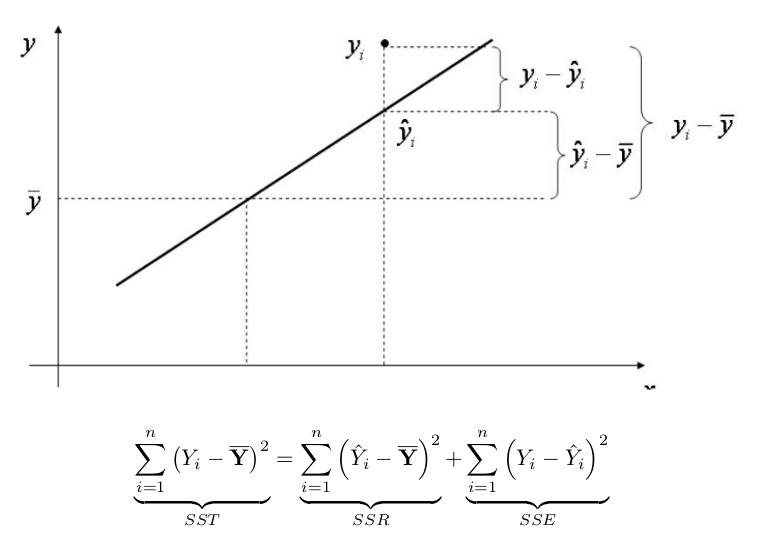
\includegraphics[scale=0.5]{anova_parts}

\todo[inline]{complete this}

